\documentclass[11pt,letterpaper]{article}
\usepackage{graphics}
\usepackage{fullpage}
\addtolength{\voffset}{0.5in}

%
%  Cool LaTeX resource:
%   http://en.wikibooks.org/wiki/LaTeX

\begin{document}
\title{Models of student learning and multimodel inference}
\author{Brett van de Sande}

\maketitle

\begin{abstract}
We compare several models of student learning of specific
skills with the goal of determining when a student has 
learned that skill.  We use Likelihood Theory to determine
which of several models best describes the acquisition
of skills associated with introductory physics.  Then we
use a multimodel approach to determine the relative probability
that a student has learned a given skill at a particular 
problem-solving step.  Finally, we relate this
approach with Hidden Markov model based approaches like
Bayesian Knowledge tracing.
\end{abstract}

\section{Introduction}

\section{A model of learning}

For each student and KC, the student has attempted some number of 
{\em steps} that involve that KC.   We will label
steps with $j$.  Usually a given step is associated
with a single user interface object (an equation, vector, etc.)  but
not always, since a student may attempt a particular problem solving
step, delete the object, and later attempt that solution step again.
Each step $j$ corresponds some some number of student-tutor 
{\em transactions}: attempts at constructing the associated object, 
or associated interactions with the Andes help system.  

%Next, we need a model of student learning for a particular KC.
%Since the policies chosen by the random-help version of Andes
%are different for each student,
%we need to determine the point of learning for each student.
For each KC and student, mark each step as ``correct'' if
the student completes the step correctly without any associated errors or 
requests for help; otherwise, the step is marked as ``incorrect.''
\label{steps} 
%
% From Kurt:
Thus, if each incorrect/correct step is marked with a 0/1, then
a single student's performance on a single KC is a bit string,
{\em exempli gratia} 00101011.

\section{Three models of learning}

In order to determine when a student has learned a given still,
we need to introduce a model of learning for that student and skill.
Ideally, the model should have the the following properties:
\label{model-criteria}
\begin{itemize} 

\item Give the probability that learning has occurred at a given step.
      See Section~\ref{multi-model}.

\item  Assuming learning has occurred at a given step, give the 
     associated increase in performance and 
     the rate of errors after learning.

\item Match well with actual student data.
      See Section~\ref{model-selection}.

\end{itemize}
%
We will consider three candidate models:  the ``step model,'' 
the logistic function, and the Bayesian Knowledge Tracing model.

A simple model that meets these criteria is the ``step model,'' defined
as:
\begin{equation}
    P_{\rm step}(j)= \left\{\begin{array}{cc}
                 g, & j<l \\
                 1-s, & j\ge L 
                 \end{array} \right. 
\end{equation}
where $L$ is the step where the student first shows mastery of the
KC, $g$ is the ``guess rate'' and $s$ is the ``slip rate'' similar
to Bayesian Knowledge tracing~\cite{anderson}.  To determine
when learning has occurred (and the associated probabilities), 
we will use a multimodel approach, 
Section~\ref{multi-model}.  The associated gain in performance
is $1-g-s$ and the error rate after learning is simply $s$ in this
model.  Thus, we can satisfy both criteria with this model.

Another model that is frequently used in this context~\cite{logit} 
is a logistic model,
%
\begin{equation}
    P_{\rm logit}(j)= \frac{1}{1+\exp\left(-b (j-L)\right)} \; .
\end{equation}
%
It is natural to associate $L$ with the moment of learning.  However,
the finite slope $P_{\rm logit}(j)$ means that learning may occur
in a range of roughly $1/b$ steps before and after $L$.  For instance,
one could associate the probability of learning during step $j$ with
the slope of $P_{\rm logit}(j)$.  For  
$P_{\rm logit}(j)$, the gain in performance is always 1 and the final error
rate is always 1.  Thus, although we can satisfy the first
criterion, the second criterion is difficult to satisfy with this model.

The third model is the Bayesian Knowledge Tracing (bkt) model~\cite{anderson}.
Although it is usually expressed as a Markov model, the solution of
this model is an exponential function (see Appendix~\ref{bkt}),
%
\begin{equation}
         P_{\rm bkt}(j) = 1-P(S) -A e^{-\beta j} \; .
\end{equation}
%
One central assumption of bkt is that, given that learning
has not already occurred, mastery is {\em equally probable} on each step.
This assumption of equal probability does not match well with 
the goal of determining empirically the steps where learning has actually occurred.
On the other hand, this model does provide initial and final
error rates.  Thus, for $P_{\rm bkt}(j)$, the second criterion is 
satisfied, but the first criterion is problematic.

\section{Model selection using AIC}
\label{model-selection}

Although this will not determine our choice of model, it 
would be reassuring to know whether the step model 
describes the student data as well (or better than) the
other two models.  For this, we believe that the Akaike Information 
Criterion (AIC) is the most appropriate metric~\cite{akaike,aicbook}.

\subsection{Method}

We examined log data from 12 students taking an intensive
summer course in 2011 at St.\ Anselm College.  The course
covered the same content as a normal two-semester introductory
course.  Log data was recorded as students solved homework 
problems while using the Andes intelligent tutor homework system.
231 hours of log data were recorded.
%, covering 85,744 transactions, and 26,204 student steps.  
Each step was assigned to one or more different KC's.  
The dataset contains a total of 2017 distinct
student-KC pairs covering a total of 245 distinct KC's.
Most KC's are associated with physics
or relevant math skills while others we associated with 
Andes conventions or user-interface actions (such as, notation
for defining a variable). 

\subsection{Analysis}

Since the goodness of fit criterion, AIC, is valid in the limit 
of many steps, we include only student-KC 
pairs that contained 10 or more turns, reducing the number of 
student-KC pairs to 267, covering 38 distinct KC's.
We determined the correctness of each step (Section~\ref{steps}),
assigning a 1 if the step is correct or 0 if it is not.
Thus, for each student-KC pair, we construct bit string, {\em exempli gratia},
001001101.  This bit string was then fit to each of the three models,
$P_{\rm step}(j)$, $P_{\rm logit}(j)$, and $P_{\rm bkt}(j)$ by
maximizing the associated log likelihood.  
%This determines the free parameters in each model. 
We then calculated the corrected AIC score, AIC$_{\mathrm c}$~\cite{aicbook} 
for each fit.  
Finally, we calculated the Akaike weights, $w_{\mathrm logit}$,
$w_{\mathrm step}$, and $w_{\mathrm bkt}$ for each student-KC pair.  
The Akaike weight represents the relative probability that
a particular model in a given set of models most closely matches
the true model that has actually generated the data.
The weights are normalized so that 
%
\begin{equation}
   1=w_{\mathrm logit}+ w_{\mathrm step} + w_{\mathrm bkt} \; .
\end{equation}
%\
A scatter plot of the weights is shown in Fig.~\ref{scatter1}.
Since we are fitting to an average of 16 data points in
each fit, we expect that AIC$_{\mathrm c}$ would not strongly
discriminate between the models.  It is only by examining
hundreds of student-KC pairs that one might find that
one model is statistically favored over the other two..  However, this is not what
we found; instead, we see that $P_{\rm bkt}$ is strongly disfavored 
over the other two.

\begin{figure}
  \centering 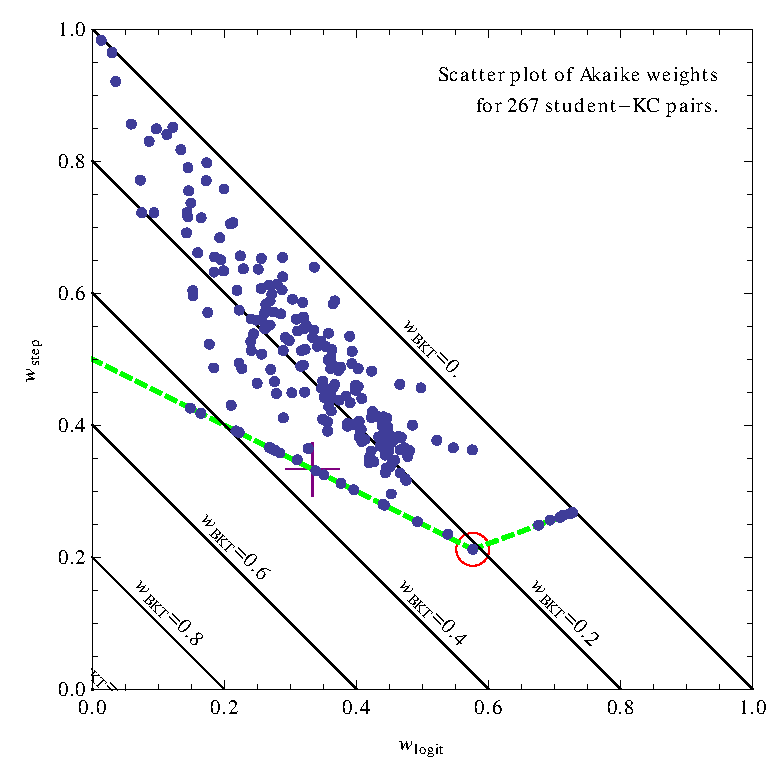
\includegraphics{scatter-weights.eps}
  \caption{Akaike weights for the three models, $P_{\rm step}$,
   $P_{\rm logit}$, and $P_{\rm bkt}$, when fit to 267
   student-KC pairs from an introductory physics course.
   The model $P_{\rm bkt}$ seems to be highly disfavored over
   the other two models; however, we believe this result
   to be spurious.} \label{scatter1}
\end{figure}

To further investigate this situation, we constructed an
artificial dataset containing 100 random bit strings (each
step has 50\% probability of being ``correct'') of 100 steps each.
This dataset corresponds to a model of the form
%
\begin{equation}
        P_{\mathrm random}(j)=1/2 \; .
\end{equation}
%
We then repeated our analysis of the three models using this
dataset.  In this
case, one expects that all three models should perform equally
well since all three can match (with suitable choice
of parameters) the known correct model $P_{\mathrm random}(j)$.
Thus, we would expect a scatter plot of the Akaike weights to 
center around 
$w_{\mathrm logit}=w_{\mathrm step}=w_{\mathrm bkt}=1/3$.
Instead, we see that $P_{\rm step}$ is highly favored over
the other two; see Fig.~\ref{scatter2}.  
This indicates that there are large non-leading
corrections to the AIC$_{\mathrm c}$ that have not been
taken into account.  Burnham \& Johnson conclude 
that there is more work to be done in this area~\cite[p.~380]{aicbook}: 
``Operating characteristics
of AIC-based model selection for count-type data need more 
more study for small sample sizes.''

\begin{figure}
  \centering 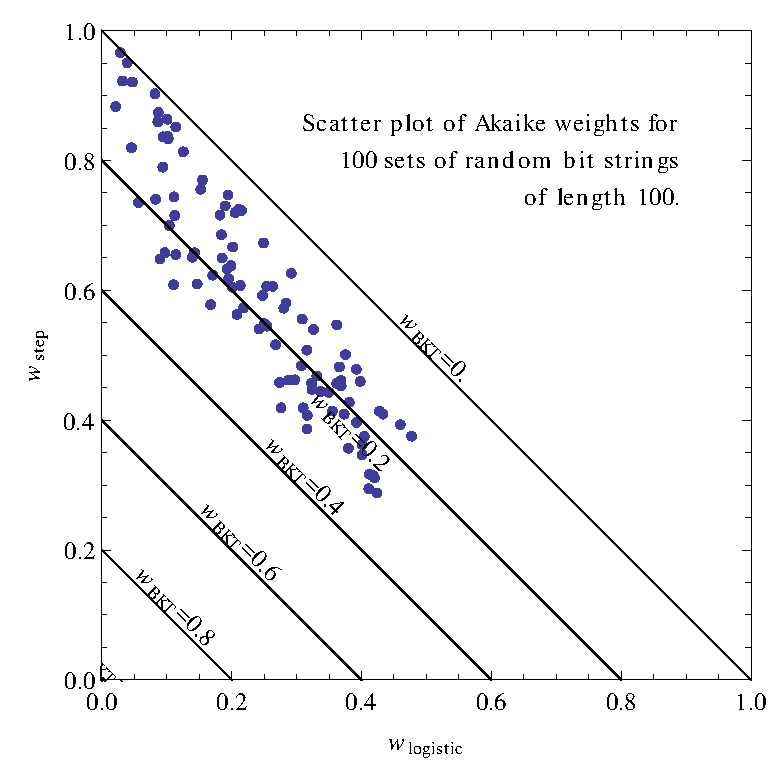
\includegraphics{scatter-random-weights.eps}
  \caption{Akaike weights for the three models, $P_{\rm step}$,
   $P_{\rm logit}$, and $P_{\rm bkt}$, when fit to randomly
   generated data.  For this dataset, each model should perform
   equally well; the large bias in favor of one model indicates
   that  AIC$_{\mathrm c}$ is failing.}\label{scatter2}
\end{figure}

\subsection{Summary}

In conclusion, the most powerful technique for model selection,
AIC, fails to to properly distinguish models when the random
variable (the dataset) is binary-valued (Bernoulli trials),
the sample sizes are small (10 to 100 points), and the models
have very different functional forms.  Since the use of such
models is foundational to KC-based approaches to Educational
Data mining, we believe that it is imperative that this issue 
be resolved.

Demonstrating that the step model fits student data as well as,
or better than, the other two would be an
{\em ex post facto} justification for using that model.  
However, the use of the step model is primarily justified
by the first two criteria listed in Section~\ref{model-criteria}.
In Section~\ref{multi-model}, we show how AIC-based methods
can yield the probability that learning has occurred during given step.

\section{Multi-model approach}
\label{multi-model}

We need to determine the step where a student has learned a given
skill.  Our strategy is to take the step model, $P_{\rm step}(j)$, 
and treat $L$ is a constant, yielding a set of sub-models, one for each $L$.
We then fit each of the sub-models to the student data, obtaining an
AIC value.  Finally, we find the Akaike weighs for each of the
sub-models.  The Akaike weights gives that probability that learning
occurred at a particular step.

\begin{figure}
  \centering 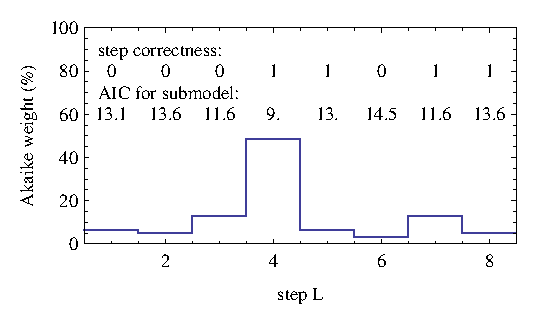
\includegraphics{step-weights.eps}
   \caption{Akaike weights for the step model $P_{\rm step}(j)$
      where $L$ is fixed.  This gives the relative probability that
      the student learned the KC just before step $L$.}
    \label{step-weights}
\end{figure}

Let us illustrate this technique with a simple example.  Suppose the 
bit-string for a particular KC is 00011011 (8 opportunities).
We fit this data to 8 sub-models, corresponding to $L\in\{1,2,\ldots,8\}$,
using maximum likelihood.  The AIC values are 
%
\begin{tabular}
   13.1, 13.6, 11.6, 9.0, 13.0, 14.5, 11.6, 13.6
\end{equation}
%
Not suprisingly, the best fit (lowest AIC) corresponds to the first
1 in the dataset at step 4.  From this, we calculate the Akaike weights
$w_L$; see Fig.~\ref{step-weights}.  

Note that $L=1$ correspon<ds to the student having ``learned the skill'' 
some time before the first step.  That is to say, they don't acquire 
the skill while using the tutor system.
Thus, $w_{L=1}$ should be interpreted as the relative probability
that no learning has occurred while using the tutor system.




%%%%%%%%%%%%%%%%%%%%%%%%%%%%%%%%%%%%%%%%%%%%%%%%%%%%%%%%%%%%%%%%%%
\appendix
\section{Bayesian Knowledge tracing}
\label{bkt}

The Bayesian Knowledge tracing model~\cite{anderson} has four parameters:
%
\begin{itemize}
   \item $P_0$ is the initial probability of knowing a skill.
   \item $P(G)$ is probability of guessing correctly, if the student        
         doesn't know the skill.
   \item $P(S)$ is probability of slips, if student does know the skill.
   \item $P(L)$ is probability of learning the skill if the student 
         does not know the skill.  Note that this is assumed to 
         be constant over steps.
\end{itemize}
%
Let $P_j$ be the probability that the student knows the skill at 
step $j$. According to the model,  $P_j$ can
be determined in terms of the previous opportunity:
%
\begin{equation}
          P_j = P_{j-1} + P(L)\left(1-P_{j-1}\right)
\end{equation}
%
According to this model, the probability that the student actually gets
opportunity $j$ correct is:
%
\begin{equation}
        P_{\rm bkt}(j) = P(G)\left(1-P_j\right) + 
                     \left(1-P(S)\right) P_j \label{pnc}
\end{equation}
%
(Unlike the four model parameters above, there isn't a consistent
notation for $P_{\rm bkt}(j)$ in the literature.)
This model can be exactly solved with solution: 
%
\begin{equation}
            P_j = 1-\left(1-P(L)\right)^j\left(1-P_0\right)
	    \label{sol}
\end{equation}
%
%
Substituting (\ref{sol}) into (\ref{pnc}), we get:
%
\begin{equation}
         P_{\rm bkt}(j) = 1-P(S) -\left(1-P(S)-P(G)\right) \left(1-P_0\right)
                   \left(1-P(L)\right)^j \label{pncsoln}
\end{equation}
%
Note that the functional form of $P_{\rm bkt}(j)$ is a function of {\em three}
parameters:  $P(S)$, $P(L)$, and $\left(1-P(S)-P(G)\right) \left(1-P_0\right)$.
This degeneracy of the model was first noticed by Beck and 
Chang~\cite{beckchang}.  In their paper, they notice that multiple
combinations of $P(G)$ and $P_0$ give exactly the same $P_{\rm bkt}(j)$, but
fail to explain why this is the case.

\begin{figure}
  \centering 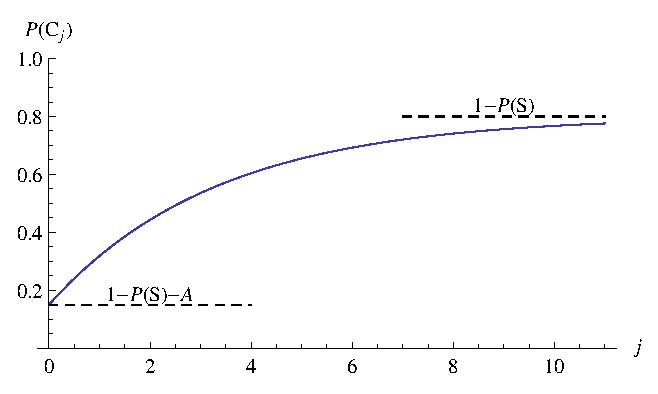
\includegraphics{exponential.eps}
   \caption{The graph of the solution of the Bayesian Knowledge
     Tracing model.}
    \label{bkt-function}
\end{figure}

The functional form of (\ref{pncsoln}) is an exponential.
If we define 
$A=\left(1-P(S)-P(G)\right) \left(1-P_0\right)$ and
$\beta=-\log(1-P(L))$, then we can rewrite (\ref{pncsoln}) in 
a clearer form:
%
\begin{equation}
         P_{\rm bkt}(j) = 1-P(S) -A e^{-\beta j}
\end{equation}
%
In conclusion, Bayesian Knowledge tracing is equivalent to using
an exponential function with three parameters to fit the student data;
see Fig.~\ref{bkt-function}


%Equations (1) and (2) of \cite{brunskill} 
%are equivalent to the first three equations in \cite{baker}
%\begin{eqnarray}
%   P(L_n|\mbox{correct}) &=& P(T)+\frac{\left(1-P(T)\right) P(L_{n-1})
%          \left(1-P(S)\right)}
%               {P(L_{n-1})\left(1-P(S)\right)+\left(1- P(L_{n-1})\right) P(G)}\\
%   P(L_n|\mbox{incorrect}) &=& P(T)+\frac{\left(1-P(T)\right) P(L_{n-1})
%          \P(S)\right}
%               {P(L_{n-1})P(S)+\left(1- P(L_{n-1})\right) \left(1-P(G)\right)}\\
%with the substitution:
%
%\begin{equation}
%         P(L_{n-1}) \to P(T)+\left(1-P(t)\right) p(L_t)
%\end{equation}
%
%This equivalence is from changing the order of updating
%student mastery and updating the estimate based on student
%response, as noted by the authors.  However, this raises
%a question for Equations (3) and (4) of \cite{brunskill}.
%Should the probability be taken before or after updating the
%student mastery:



\begin{thebibliography}{9}

\bibitem{anderson} 
  Corbett, A.\ T., Anderson, J.\ R. Knowledge Tracing:  Modeling 
the Acquisition of Procedural Knowledge.  \emph{User Modeling and
 User-Adapted Interaction}, 1995, 4, 253--278.

\bibitem{beckchang}
  Beck, J.\ E., Chang, K.-m.\ Identifiability: A Fundamental Problem of
  Student Modeling.
  \emph{Proceedings of the $11^{th}$ International Conference on User 
    Modeling}, 2007.

\bibitem{baker} Baker, R, Corbett, A., Aleven, V.,  Improving Contextual 
    Models of Guessing and Slipping with a Truncated Training Set. 
    First International Conference on Educational Data Mining. 2008. 

\bibitem{brunskill}
   Lee, J.\ I., Brunskill, E.\ The impact of Individualizing Student 
  Models on Necessary Practice Opportunities.  EDM, 2012.

\bibitem{logit}
  Ken Koedinger paper, other papers, using logistical regression.
  Min Co-author on some?

\bibitem{akaike}
   Akaike original paper

\bibitem{aicbook}
   Burnham \& Johnson book

\end{thebibliography}




\end{document}